%%%%%%%%%%%%%%%%%%%%%%%%%%%%%%%%%%%%%%%%%
% Kieker Monitoring Component
% 
% $Date$
% $Rev$:
% $Author$


\chapter{\KiekerMonitoringPart{} Component}\label{chap:componentsMonitoring}

\NOTIFYBOX{The Java sources of this chapter can be found in the %
\file{\customComponentsBookstoreApplicationDirDistro{}/} directory of the %
binary release.}

\section{\KiekerMonitoringPart{} Configuration}\label{sec:monitoring:configuration}

\KiekerMonitoringPart{} is being configured by a properties file. A sample %
configuration file, which can be used as a template for custom configurations, %
is provided by the file \file{\monitoringPropertiesFile} in the directory %
\dir{\KiekerDir/META-INF/} of the binary release %
(see Section~\ref{sec:example:downloadInstall}). %

In order to use a custom configuration file, the file location needs to be passed to %
the JVM using the parameter \textit{kieker.monitoring.properties} as follows:

\setBashListing
\begin{lstlisting}[caption=,label=lst:monitoringPropertiesPassedToJVM]
#\lstshellprompt# java	#\textbf{-Dkieker.monitoring.properties=}#<ANY-DIR>/my.kieker.monitoring.properties #[\ldots]#
\end{lstlisting}

\noindent Appendix~\ref{sec:appdx:monitoringproperties} lists this file with a documentation 
of all available properties. If no configuration file %
is passed, a default configuration (according to the sample file) is being %
used by \KiekerMonitoringPart{}. %

\section{Monitoring Controller}\label{sec:componentsMonitoring:monitoringController}

The \class{MonitoringController} constructs and controls a \KiekerMonitoringPart{} %
instance and provides methods to, among others, log monitoring records %
(\method{newMonitoringRecord}) employing the configured monitoring log writer and %
to retrieve the current timestamp (\method{currentTimeNanos}). %
The class is implemented employing the singleton pattern. The singleton instance %
can be retrieved by calling the static method \method{getInstance}. %
Figure~\ref{fig:monitoringController:classdiagram} shows %
a class diagram of the class \class{MonitoringController} including the methods 
just mentioned. The \class{MonitoringController} reads the configuration %
file, as described in Section~\ref{sec:monitoring:configuration}.


\begin{figure}[H]\centering
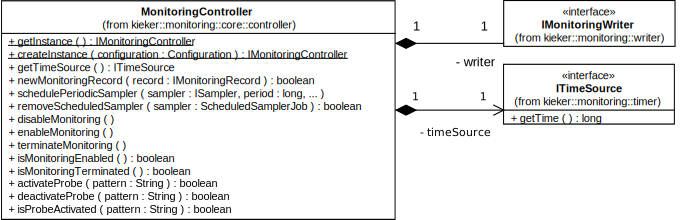
\includegraphics[scale=0.7]{images/kieker_monitoringControlleruserguide-simplified}
\caption{Class diagram of the \class{MonitoringController} (including selected methods)}
\label{fig:monitoringController:classdiagram}
\end{figure}


\section{Monitoring Records}\label{sec:componentsMonitoring:monitoringRecords}

Monitoring records are objects that contain the monitoring data, as mentioned %
in the previous chapters. Typically, an instance of a monitoring record is %
constructed in a monitoring probe (Section~\ref{sec:monitoring:probe}), %
passed to the monitoring controller (Section~\ref{sec:componentsMonitoring:monitoringController}), %
serialized and deserialized by a monitoring %
monitoring log writer (Section~\ref{sec:monitoring-log-writers}) and a
monitoring log reader (Section~\ref{sec:analysis:reader}), and provided to the %
analyis plugins (Section~\ref{sec:analysis:consumer}) %
by the analysis controller (Section~\ref{sec:analysis:controller}). %
Figure~\ref{fig:KiekerCommunicationDiagram} illustrates this life cycle of a monitoring %
record. %

In Chapter~\ref{chap:example}, we've already introduced and used the monitoring %
record type \class{OperationExecutionRecord}. \Kieker{} allows to use custom %
monitoring record types. Corresponding classes must implement the %
interface \class{IMonitoringRecord} shown in Figure~\ref{sec:monitoringrecord:interfacesAndImplementingClasses}. %
The methods \method{initFromArray}, \method{toArray}, \method{getValueTypes} %
are used for serialization and deserialization of the monitoring data contained %
in the record. The method \method{setLoggingTimestamp} is used by the monitoring controller to %
store the date and time when a record is received by the controller. %
The \method{getLoggingTimestamp} can be used during analysis to retrieve %
this value. \KiekerMonitoringPart{} provides the abstract class %
\class{AbstractMonitoringRecord} (Figure~\ref{sec:monitoringrecord:interfacesAndImplementingClasses}) %
which already implements the methods to maintain the logging timestamp. 

\begin{figure}[h]\centering
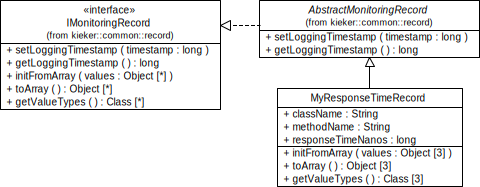
\includegraphics[scale=0.7]{images/kieker_MyRTRecord-modified}
\caption{Class diagram with the \class{IMonitoringRecord} interface, the abstract %
class \class{AbstractMonitoringRecord}, and a custom monitoring record type %
\class{MyResponseTimeRecord}}
\label{sec:monitoringrecord:interfacesAndImplementingClasses}
\end{figure}

\noindent In order to implement your own monitoring record type, you need to:

\begin{enumerate}
\item Create a class that extends \class{AbstractMonitoringRecord}  and
\item Override the methods \method{initFromArray}, \method{toArray}, \method{getValueTypes}.
\end{enumerate}

\noindent The class \class{MyResponseTimeRecord}, shown in the class diagram in %
Figure~\ref{sec:monitoringrecord:interfacesAndImplementingClasses} and in %
Listing~\ref{listing:MyRecord}, is an example of a custom monitoring record type %
that can be used to monitor response times of method executions.

\setJavaCodeListing
\lstinputlisting[caption=MyResponseTimeRecord.java, label=listing:MyRecord]{\customComponentsBookstoreApplicationDir/src/bookstoreApplication/MyResponseTimeRecord.java}


\section{Monitoring Probes}\label{sec:monitoring:probe}

The probes are responsible for collecting the monitoring data and passing this %
monitoring data to the monitoring controller. %
In Chapter~\ref{sec:example:monitoring}, we have already demonstrated how to %
manually instrument a Java application. Listing~\ref{listing:cuttingBookstore} %
shows a similar manual monitoring probe which uses the monitoring record type %
\class{MyResponseTimeRecord} defined in the previous Section~\ref{sec:componentsMonitoring:monitoringRecords}.

% Make sure that this listing will be modified, once the sourcecode changes!!!
% It must show the whole monitoring of the bookstorecall, from getting the first time to persisting of the record!!
\lstinputlisting[firstline=14, lastline=23, firstnumber=14, caption=Excerpt from Bookstore.java, label=listing:cuttingBookstore]{\customComponentsBookstoreApplicationDir/src/bookstoreApplication/Bookstore.java}

\noindent In order to avoid multiple calls to the \method{getInstance} method of the %
\class{MonitoringController} class, the singleton instance should be stored %
in a final static variable, as shown in Listing~\ref{listing:cuttingBookstore:finalStaticController}.

\lstinputlisting[firstline=9, lastline=10, firstnumber=9, caption=Singleton instance of the monitoring controller stored in a final static variable (excerpt from Bookstore.java), label=listing:cuttingBookstore:finalStaticController]{\customComponentsBookstoreApplicationDir/src/bookstoreApplication/Bookstore.java}

\noindent When manually instrumenting an application, the monitoring probe is implemented %
by mixing monitoring logic with business logic, which is often not desired since %
the resulting code is hardly maintainable. %
Many middleware technologies, such as Java~EE Servlet~\cite{JavaServletTechnology-WebSite}, %
Spring~\cite{Spring-WebSite}, and %
Apache~CXF~\cite{CXF-WebSite} provide interception/AOP~\cite{Kiczales1997} interfaces %
which are well-suited to implement monitoring probes. AspectJ~\cite{AspectJ-WebSite} allows to %
instrument Java application without source code modifications. %
Chapter~\ref{chap:aspectJ} provides probes based on these technologies allowing to %
monitor trace information in distributed applications. 

\section{Monitoring Log Writers}\label{sec:monitoring-log-writers}

Monitoring log writers serialize monitoring records to the monitoring log and  % and persist the recorded informations into files, databases etc. %
must implement the interface \class{IMonitoringLogWriter}. The monitoring %
controller passes the received records to the writer by calling the method %
\method{newMonitoringRecord}. Writers can use the methods to serialize the %
record contents, as described in Section~\ref{sec:componentsMonitoring:monitoringRecords}. 

Figure~\ref{figure:monitoringLogWritersHierarchy} shows the monitoring writers %
already implemented in \KiekerMonitoringPart{}. The writers \class{AsyncFsWriter}, %
\class{SyncFsWriter}, \class{AsyncDbWriter}, and \class{SyncDbWriter} can be used %
to store monitoring records to filesystems and databases respectively. %
The variants with the prefix \class{Async} are implemented using asynchronous %
threads that decouple the I/O operations from the control flow of the %
instrumented application. % 
The \class{AsyncFsWriter} is the default writer which has already been used in %
Section~\ref{sec:example:monitoring}. %
Currently, the database writer only supports the record type \class{OperationExecutionRecord}. %

The \class{AsyncJMSWriter} writes records to a JMS (Java Messaging Service~\cite{JMS-WebSite}) queue. %
This allows to implement on-the-fly analysis in distributed systems, i.e., analysis while %
continuously receiving new monitoring data from an instrumented application potentially %
running on another machine. A brief description of how to use the \class{AsyncJMSWriter} %
can be found in Appendix~\ref{appendix:usingJMS}. %
The \Kieker{} web site provides an example for this. %

% This is the diagram with the hierarchy of the writers.
\begin{figure}[H]
\begin{centering}
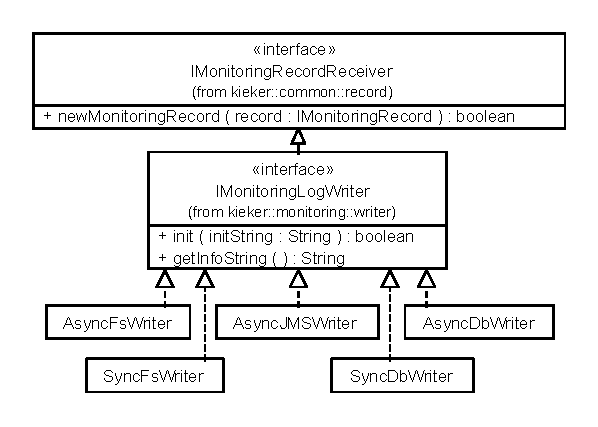
\includegraphics[width=0.5\textwidth]{images/kieker_writerimplsuserguide-modified}
\caption{Interface \class{IMonitoringLogWriter} and  the implementing classes}
\label{figure:monitoringLogWritersHierarchy}
\end{centering}
\end{figure}

\noindent Listing~\ref{listing:MyWriter} shows a custom writer \class{MyPipeWriter} which uses a named pipe to %
write the given records into a buffer located in the memory. The source code of %
the class \class{MyPipe} is listed in Appendix~\ref{appendix:pipeListings}. %

\setJavaCodeListing
\lstinputlisting[caption=MyWriter.java, label=listing:MyWriter]{\customComponentsBookstoreApplicationDir/src/bookstoreApplication/MyPipeWriter.java}

\noindent The monitoring writer to be used is selected and configured by the \KiekerMonitoringPart{} %
configuration properties (Section~\ref{chap:componentsMonitoring}) %
\textit{monitoringDataWriter} and \textit{monitoringDataWriterInitString}. %
Listing~\ref{lst:monitoringwriter:MyWriter} demonstrates how to use the custom %
writer \class{MyPipeWriter} defined above. In this example, the pipe name is %
passed as the property value \textit{monitoringDataWriterInitString}.

\setBashListing       
\begin{lstlisting}[label=lst:monitoringwriter:MyWriter]
monitoringDataWriter=bookstoreApplication.MyPipeWriter
monitoringDataWriterInitString=pipeName=somePipe
\end{lstlisting}

\noindent Notice, that we decided to use \class{Object} arrays as the data structure of the %
monitoring log in order to demonstrate the use of the \method{toArray} and %
\method{initFromArray} (in Section~\ref{sec:analysis:reader}) methods. %
Alternatively, we could have used \class{IMonitoringRecord} as the data structure %
used by the pipe. %